\documentclass[a4paper]{article}

\usepackage{xcolor}
\usepackage{fancyhdr}
\usepackage{listings}
\usepackage{graphicx}
\usepackage[utf8]{inputenc}
\usepackage{multirow}
\usepackage{wrapfig}
\usepackage{enumitem}
\lstset{frameround=fttt,numbers=left,breaklines=true, extendedchars=true}

\hyphenation{be-schre-ven}

\addtolength{\textwidth}{1.5in}
\addtolength{\topmargin}{-.875in}
\addtolength{\oddsidemargin}{-.75in}
\addtolength{\evensidemargin}{-.75in}
\addtolength{\textheight}{1.75in}

\newcommand{\todo}[1]{\textcolor{red}{[#1]}}
\lhead{Open Universiteit}
\chead{IM0202, Software evolution}
\rhead{Assignment 2}

\begin{document}
\pagestyle{fancy}

\section*{Studentgegevens}
\begin{description}
	\item [Cursuscode]: IM0202
	\item [Naam]: Ewoud Westerbaan
	\item [Studentnummer]: 852069942
	\item [Naam]: Martin de Boer
	\item [Studentnummer]: 837372832
\end{description}

\section{Samenwerking}
De eerste iteratie is gebouwd op basis van een experiment van Martin, die tijdens de kerstdagen al was begonnen. Deze uitkomst hebben we als basis genomen en bepaald wat toegevoegd en/of aangepast zou moeten worden. Vooral Martin heeft hier veel werk in verzet.
Het cache mechanisme en een eerste versie van een zelfgemaakte boxplot is door Ewoud gemaakt, maar deze boxplot is later door Martin nog iets verbeterd. Rascal biedt nog geen boxplot aan (deze is nog in experimentele fase).


\section{Aannames}
\begin{description}
\item[Data is consistent] We gaan ervan uit dat de data waar we de visualisatie op maken, dezelfde is als de data uit assignment 1. Voor de visualisatie gebruiken we niet de duplicatiemetrieken.
\item[Kleurenblindheid en grijstinten] We gaan er van uit dat mensen met kleurenblindheid wel grijstinten kunnen onderscheiden.
\end{description}

\section{Criteria} \label{Criteria}
Criteria met betrekking tot esthetiek en gebruiksvriendelijkheid:
\begin{enumerate}
\item Voorkom vertekeningen in waarnemingen \cite{tufte2014visual} p.56. Hiermee wordt bedoeld dat de fysieke grootte van een object in verhouding moet staan met de werkelijke numerieke waarde. Een verkeerde verhouding noemt Tufte de `Lie Factor'.
\item Aantal informatiedragende dimensies mag niet groter zijn dan het aantal dimensies in de data \cite{tufte2014visual} p.71. Tufte geeft aan dat het gebruik van meerdere dimensies ten opzichte van het aantal dimensies dat de data bevat, leidt tot misleiding en fouten in het ontwerp.

\item Stephen Few geeft enkele criteria met betrekking tot kleurgebruik \cite{B}:
\begin{enumerate}[nosep]
\item Gebruik zachte kleuren, tenzij je iets uit wilt lichten;
\item Gebruik dezelfde kleur, tenzij dit geassocieerd wordt met een andere betekenis; 
\item Gebruik een enkele, neutrale achtergrondkleur.
\end{enumerate}

\item Ben Shneiderman heeft voor gebruiksvriendelijkheid de `Visual Information-Seeking Mantra` beschreven. Deze theorie houdt in dat eerst een overzicht gegeven moet worden, en men vervolgens moet kunnen inzoomen en filteren. Details moeten op aanvraag beschikbaar zijn \cite{A}. Tufte geeft ook een zelfde principe: `reveal the data at several levels of detail, from a broad overview to the fine structure` \cite{tufte2014visual} p. 13.

\item De performance moet acceptabel zijn. We geven hier geen richtlijnen voor performance, maar gebruikers moeten niet al te lang wachten voor de visualisatie geladen is.
\end{enumerate}


\section{Selectie van de architectural view}
Het doel van onze visualisatie is de kwaliteit van een applicatie op basis van complexiteit en unit size te laten zien voor ontwikkelaars in een nieuwbouw- of beheerfunctie. In Figuur \ref{fig:overview} is een overzicht van de visualisatie te zien.

\begin{figure}[h]
  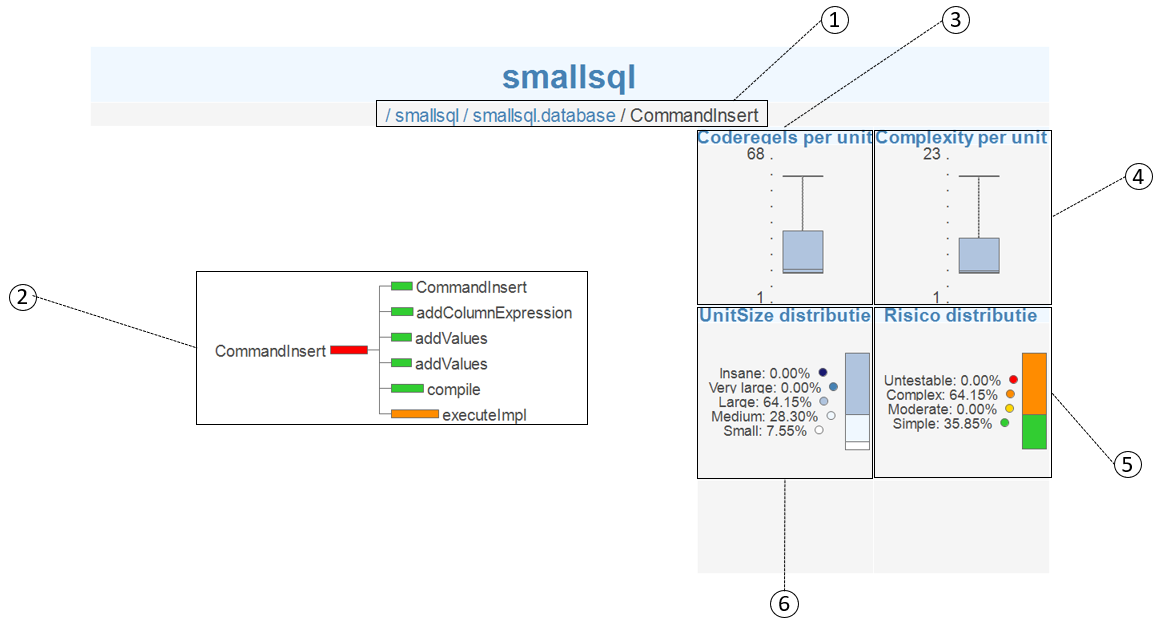
\includegraphics[width=0.8\linewidth]{images/overview_with_numbers.png}
  \caption{Overview}
  \label{fig:overview}
\end{figure}
 
Het grootste deel van het scherm bestaat uit een tree view. De nodes representeren een project, packages, klassen en units (methodes en constructors). Bij het opstarten wordt het project als parent node met daaronder de packages weergegeven (het meest abstracte niveau). We hebben voor een tree view gekozen, omdat we daar meerdere metrieken in kwijt kunnen; de complexiteitwaarde wordt getoond in kleur, unit size in grootte, en de hiërarchie van de applicatie doormiddel van de structuur van de figuur (Figuur \ref{fig:overview}: \textcircled{2}). 
\begin{figure}[h]
  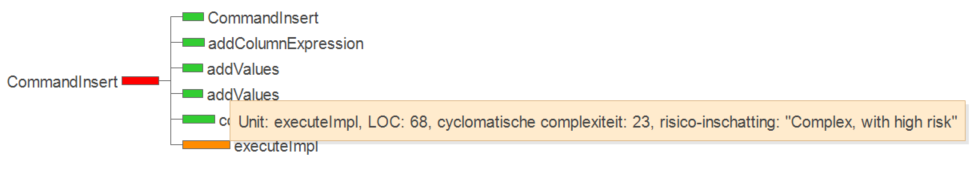
\includegraphics[width=\linewidth]{images/treeview_with_popup.png}
  \caption{Treeview met popup}
  \label{fig:treeview_popup}
\end{figure}

\begin{wrapfigure}{r}{0.5\textwidth}
\begin{center}
  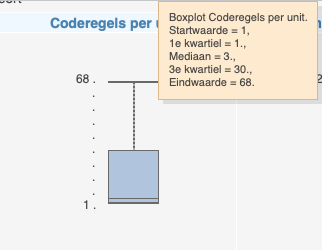
\includegraphics[width=0.35\textwidth]{images/boxplot_popup.png}
  \end{center}
  \caption{Boxplot met popup}
  \label{fig:boxplot_popup}
\end{wrapfigure}
Om het overzicht te bewaren, laat de tree view niet direct waardes zien, maar zijn deze in een popup van een element (package, klasse of methode) te zien wanneer men met de muis hier overheen gaat, zie Figuur \ref{fig:treeview_popup}. Interactiviteit is ingebouwd op de volgende manieren: 1) men kan inzoomen door op een klasse of package te klikken 2) men kan uitzoomen door een shift+klik te doen op een parent node. Het meest gedetailleerde niveau is een methode of constructor, zoals te zien in Figuur \ref{fig:treeview_popup}.

Om een overzicht te geven waar men zich in de hiërarchie van de applicatie bevindt, wordt een kruimelpad getoond (Figuur \ref{fig:overview}: \textcircled{1}). Men kan uitzoomen door op het gewenst niveau te klikken.


De rechterkant bevat een paneel met inzicht in de verdeling van waardes. Een stacked bar biedt inzicht in de verhouding van de classificaties in het \mbox{geselecteerde} niveau. Naast deze stacked bar zijn de percentages zichtbaar. Een boxplot geeft de verdeling van waardes. Een mouse-over laat een popup zien van de waardes (startwaarde, 1e kwartiel, mediaan, 3e kwartiel en eindwaarde), zie Figuur \ref{fig:boxplot_popup}.
Een stacked bar en boxplot worden getoond voor complexiteit en unit size (Figuur \ref{fig:overview}: \textcircled{3}) en laten waardes zien voor het geselecteerde niveau.

De visualisatie hebben we ook bruikbaar gemaakt voor mensen die minder goed kleuren kunnen onderscheiden. Door de applicatie met een extra parameter ‘BW’ (indicatie kleurenpallet) op te starten, worden de kleuren rood, oranje, geel en groen vervangen door grijstinten, zie Figuur \ref{fig:overview_blackwhite}.
\begin{figure}[h]
\centering
  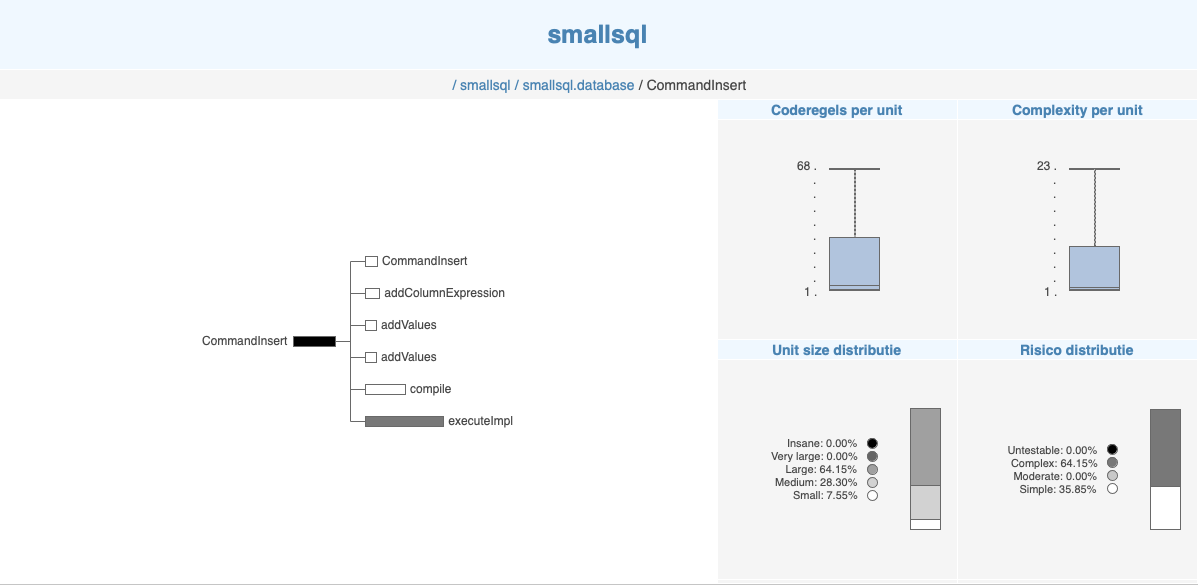
\includegraphics[width=0.8\linewidth]{images/overview_blackwhite.png}
  \caption{Overview in grijstinten}
  \label{fig:overview_blackwhite}
\end{figure}

\section{Resultatenanalyse}
Met het voorkomen van vertekeningen van waarnemingen (criterium 1 in Sectie \ref{Criteria}) hebben we beperkt rekening kunnen houden. De tree view wordt onleesbaar als we dit wel zouden toepassen. Een voorbeeld is een klasse waar een methode inzit met een unitsize van één en een methode met een unit size van 200.
Een ander voorbeeld zijn de punten aan de zijkant van de boxplot, dit zijn er altijd 10 en dat kan misleidend zijn.

Het aantal informatiedragende dimensies (criterium 2 in Sectie \ref{Criteria}) hebben we wel goed toegepast. De boxplots en stacked bars zijn een 1-dimensionale weergave van een metriek. In de tree view worden twee dimensies weergegeven doormiddel van kleur en grootte. 

De kleurstelling (criterium 3 in Sectie \ref{Criteria}) die we hebben toegepast is in de gehele visualisatie hetzelfde.  De achtergrond hebben we een neutrale kleuren gegeven, waarbij de achtergrond van de rechterkant iets donkerder is. Wij willen hiermee bereiken dat men eerst geleid wordt naar de tree view.

De `Visual Information-Seeking Mantra' (criterium 4 in Sectie \ref{Criteria}) hebben we toegepast door de visualisatie te laten starten op project niveau. Door te klikken kan men een niveau inzoomen naar package en/of klasse niveau. Het op aanvraag beschikbaar zijn van de details zit verwerkt in de visualisatie door alleen de waardes te geven van een metriek wanneer men met de muis over een boxplot van een metriek gaat (popup). Dit geldt ook voor details in de tree view.

Een acceptabele performance (criterium 5 in Sectie \ref{Criteria}) hebben we geïmplementeerd door het implementeren van een cache mechanisme. Dit cache mechanisme \mbox{schrijft} berekende data weg naar schijf en leest deze weer in bij het opstarten van de applicatie.

\bibliographystyle{abbrv}
\bibliography{verslag_assignment2}

\end{document}
